%!TEX root = ../thesis.tex

\section{背景}
近年, 様々なセンサを用いた自律移動に関する研究が活発に行われており, その中で視覚を入力としたend-to-end学習により自律走行した例もある. 例えば, Bojarskiらは\figref{Fig:bojaski}に示すシステムでカメラ画像と人が操作するステアリングの角度をend-to-end学習することで, 自律走行する手法を提案した\cite{bojaski}.

\vspace{20mm}

\begin{figure}[hbtp]
\centering
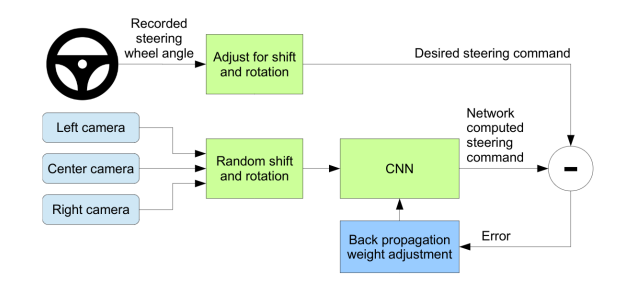
\includegraphics[keepaspectratio, scale=0.5]
{images/bojaski.png}
\caption{Training the neural network from \cite{bojaski}}
\label{Fig:bojaski}
\end{figure}

\newpage
岡田らは\figref{Fig:tsudanuma2-3}のように地図ベースのナビゲーションによる出力を模倣することで, 経路追従行動を獲得した\cite{okada-si2020}. \figref{Fig:okada-si2020}に示すような, LiDAR, オドメトリを入力としたナビゲーションの出力をend-to-endで模倣学習し, 学習後はカメラ画像を入力とした学習器の出力により, 一定の経路において周回が可能であることが確認された. 

\vspace{20mm}

\begin{figure}[h]
     \centering
     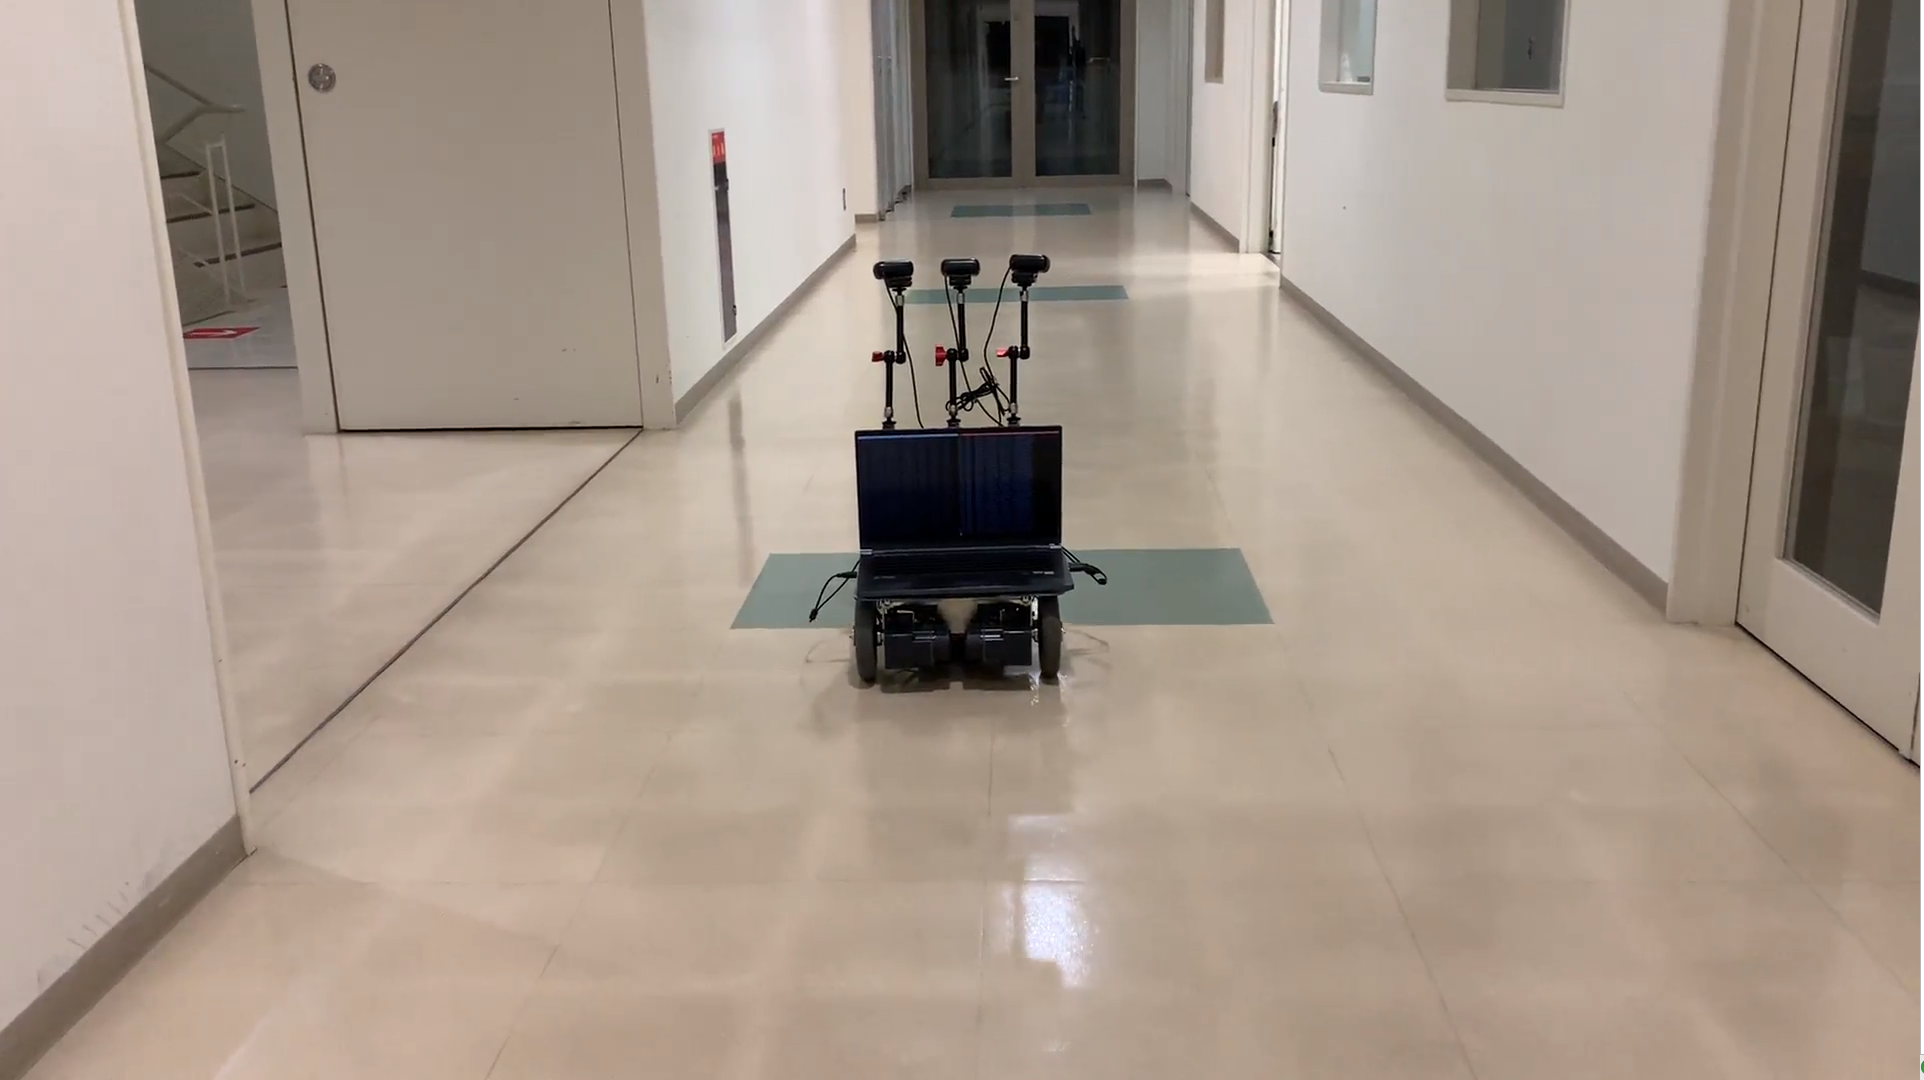
\includegraphics[keepaspectratio, scale=0.15]
     {images/tsudanuma2-3.png}
     \caption{Map based navigation using navigation indoors from \cite{okada-si2020}}
     \label{Fig:tsudanuma2-3}
     \end{figure}

\begin{figure}[h]
     \centering
     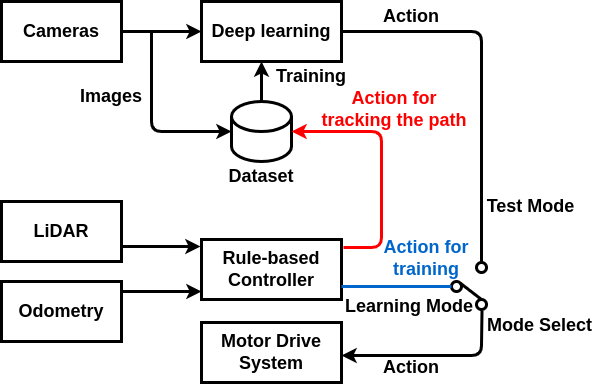
\includegraphics[keepaspectratio, scale=0.42]
     {images/okada-si2020.png}
     \caption{Systems that imitation learning for map-based navigation from \cite{okada-si2020}}
     \label{Fig:okada-si2020}
     \end{figure}

\newpage
また, 清岡ら\cite{kiyooka-si}により, \figref{Fig:kiyooka-si}に示すような手法を用いて, 経路上だけでなく経路から離れた状態も学習することが, 経路追従行動を模倣する上で有効であることが示された. 

\vspace{10mm}

\begin{figure}[h]
     \centering
     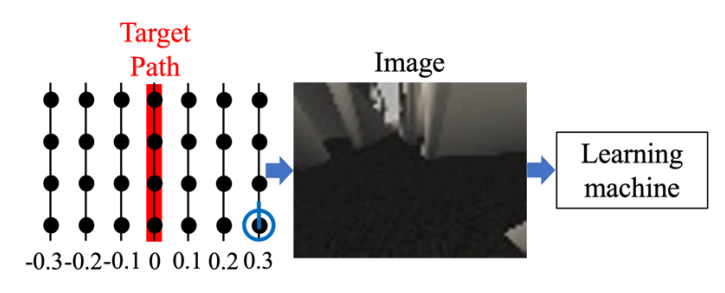
\includegraphics[keepaspectratio, scale=0.45]{images/kiyooka-si-1.png}
     \caption{Procedure for visualizing the output of the learning machine from \cite{kiyooka-si}}
     \label{Fig:kiyooka-si}
     \end{figure}

\vspace{20mm}
以上で述べたように, カメラ画像を入力とした学習器の出力により, ロボットが学習した経路を周回可能であることが示されている. \par 次に, 岡田らと清岡ら(以下「従来手法」と称する)の提案手法を基に, 新たなデータセットの収集方法を提案する.

% \newpage
% \section{関連研究}
% Yunpeng Pan\cite{batch}らは, \figref{Fig:batch1}に示すシステムと\figref{Fig:net}にのようなネットワークにより, バッチ学習とオンライン学習を用いて, 高度なセンサーを備えたモデル予測制御を模倣した. これにより, \figref{Fig:batch2}のようにオフロードでの自律走行を獲得した. 

% \begin{figure}[h]
%      \centering
%      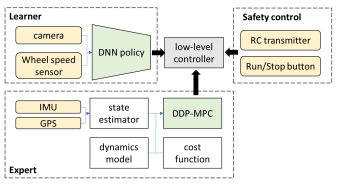
\includegraphics[keepaspectratio, scale=0.7]{images/batch1.png}
%      \caption{Yunpeng Pan and others proposed method from \cite{batch}}
%      \label{Fig:batch1}
%      \end{figure}

% \begin{figure}[h]
%      \centering
%      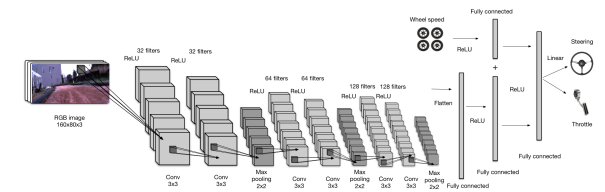
\includegraphics[keepaspectratio, scale=0.5]{images/net.png}
%      \caption{Yunpeng Pan and others proposed network from \cite{net}}
%      \label{Fig:net}
%      \end{figure}

% \begin{figure}[h]
%      \centering
%      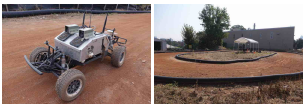
\includegraphics[keepaspectratio, scale=0.7]{images/batch2.png}
%      \caption{Autonomous off-road driving}
%      \label{Fig:batch2}
%      \end{figure}

% @misc{batch,
% author = {Yunpeng Pan and Ching-An Cheng and Kamil Saigol and Keuntaek Lee and Xinyan Yan and Evangelos A. Theodorou and Byron Boots},
% title = {"Agile Autonomous Driving using
% End-to-End Deep Imitation Learning''},
% howpublished = {},
% month = {},
% year = {},
% note = {30332–0250},
% }

\newpage
\section{目的}
本研究では, 先行研究を基にオフラインでデータを収集して学習を行う手法を提案する. これにより, 経路追従が可能であるかをシミュレータを用いた実験を通して検証する. 

\section{論文構成}
本論文の構成は以下に述べる通りである. 第1章では, 研究を行う背景や目的を述べた. 第2章では, 研究に関連する要素技術, 第3章では, 従来手法について説明する. 第4章では, 提案手法について説明し, 第5章では, 実験について説明する. そして, 第6章では, 本研究の結論を述べる. 
     
